\documentclass{beamer}

\usetheme{Warsaw}

\usepackage{mathlist}

\usepackage[utf8]{inputenc}
\usepackage{amsmath,amssymb}

\newtheorem{defi}{Définition}
\newtheorem{theo}{Théorème}
\newtheorem{coro}{Corollaire}
\newtheorem{lem}{Lemme}

%\usepackage{epic,eepic}
%\usepackage{pstricks, pst-tree}

\usepackage{times}

\usepackage{ulem}
\usepackage{crayola}

\usepackage{listings}
%\topmargin=-0.6in
\lstloadlanguages{C++}
\lstset{language=C++}
%%}

\setbeamercovered{dynamic}

\def\bxi{\boldsymbol\xi}
\def\bepsilon{\boldsymbol\epsilon}
\def\bomega{\boldsymbol\omega}
\def\aff{\operatorname{aff}}

\newcommand{\tim}[1]{\;\; \mbox{#1} \;\;}

\title[Adaptive methods]{Programmation stochastique\\SAA: méthodes adaptatives}

\author{Fabian Bastin}

\date{IFT-6512 -- Hiver 2011}

\begin{document}

\frame{\titlepage}

\begin{frame}
\frametitle{Motivation}

\underline{Reminder}: we consider the stochastic problem
\[
\textcolor{red}{\min_{z \in S} g(z) = E_P \left[ G(z, \bxi) \right]},
\]
where $z \in \rit^m$ is a vector of decision variables, $S$ is a compact subset of $\rit^m$ representing the feasible solutions, $\bxi$ is a real random vector defined on $( \Xi, \mathcal{F}, P )$ and taking values in $( \rit^k, \mathcal{B}^k )$ ($\mathcal{B}^k$ is the Borel measure), $G: \rit^m \times \rit^k \rightarrow \rit$ is a real-valued function, and $E_P[\cdot]$ is the expectation with respect to the measure $P$.

\mbox{}

Sample average approximation:
\[
\min_{z \in S} \hat{g}_N(z) = \frac{1}{N} \sum_{i = 1}^N G (z, \xi_i),
\]

\end{frame}

\begin{frame}
\frametitle{Convergence}

We have seen some consistency results for $N \rightarrow \infty$.
Moreover, the central limit theorem tells us that, if the draws are independent and identically distributed (i.i.d.) (and finite $g(z)$),
\[
\sqrt{N} [ \hat{g}_N(z) - g(z) ] \Rightarrow N(0, \sigma^2(z)),
\]
where $\sigma^2(z) = \mbox{var}(G(z,\xi))$, and $\Rightarrow$ denotes convergence in probability.

\mbox{}

This result is only valid for a given $z$.
It is necessary to set stronger conditions in order to have a functional convergence.

\mbox{}

Remark first that, under our working assumptions, $\hat{g}_N(x)$ is continuous over $S$, and can thus be considered as a point in the Banach space $C(s)$.

\end{frame}

\begin{frame}
\frametitle{Banach space $C(s)$}

$C(S)$ is the space of continuous functions $\psi: S \rightarrow \rit$,
equipped with the sup-norm $\| \psi \| := \sup_{x \in S}| \psi |$

\mbox{}

$C(S)$ is a Banach space, i.e. a normed vectorial space, complete under the distance issued from its norm.
A metric space $M$ is said complete of complete space if every Cauchy suite in $M$ has a limit in $M$ (i.e. it converges in $M$).

\mbox{}

We will extend the (pointwise) central limit theorem to a functional central limit theorem, assuming as usual that the draws are i.i.d.

\end{frame}

\begin{frame}
\frametitle{Functional central limit theorem}

Assume that the following assumptions hold:
\begin{enumerate}
\item
For all $x \in S$, the function $G(x,\cdot)$ is measurable (in other words, its expectation exists).
\item
The expectation $E_P[G(\overline{x}, \xi)^2]$ is finite for some point $\overline{x} \in S$.
\item
The Lipschitz continuity condition
\[
| G(x_1, \xi) + G(x_2, \xi) )| \leq K(\xi) \| x_1 - x_2\|,
\]
holds for a positive random variable $K(\xi)$, such that $E[K(\xi)]$ is finite, for all $x_1$, $x_2 \in S$ and almost every $\xi$.
We assume moreover that the random variable $K(\xi)$ has a finite second order moment.
\end{enumerate}

\end{frame}

\begin{frame}
\frametitle{Functional central limit theorem (cont'd)}

Under these conditions,
\[
N^{1/2} [\hat{g}_n - g] \Rightarrow Y \in C(S).
\]
With the i.i.d. condition, $Y$ is such that for any points $x_1,\ldots,x_k \in S$, the random vector $(Y(x_1),\ldots,Y(x_k))^T$ follows a multivariate normal distribution, with the covariance matrix corresponding to the covariance of the vector $(G(x_1, \xi), \ldots, G(x_k, \xi))$.

\mbox{}

In the case of global minimization, we have the following result: if $N^{1/2}(\hat{g}_N - g) \Rightarrow Y \in C(S)$ (with $\lbrace \hat{g}_n \rbrace$ and $g$ in $C(S)$, then
\[
N^{1/2}(\hat{v}_N - v^*) \Rightarrow \min_{x \in S^*} Y(x).
\]
where
\[
\hat{v}_N = \min_{x \in S} \hat{g}_N(x) \mbox{ et } v^*= \min_{x \in S} g(x).
\]

\end{frame}

\begin{frame}
\frametitle{Convergence of global solutions}

If $S^*$ is a singleton, under the previous assumptions, in the i.i.d. case,
\[
N^{1/2}(\hat{v}_n - v^*) \Rightarrow N(0, \sigma^2(x^*) ).
\]

\mbox{}

Under some additional conditions, we also have the convergence of $E[\hat{v}_N]$ to $v^*$.

\mbox{}

But all these results become difficult to extend in the case of local optimization.

\mbox{}

However, we see that the more $N$ is large, the better should be the result.
But increasing $N$ also increase the computation cost of the approximate function, as\[
\hat{g}_N(z) = \frac{1}{N} \sum_{i = 1}^N G (z, \xi_i).
\]

\end{frame}

\begin{frame}
\frametitle{External adaptive method}
%\frametitle{Convergence of global solutions (cont'd)}

What does interest us?
\[
\textcolor{red}{\min_{z \in S}}\ \hat{g}_N(z) = \frac{1}{N} \sum_{i = 1}^N G (z, \xi_i).
\]
In other terms, for a given approximation level defined by the number of random draws, it is possible to speed up the first iterations of the optimization process by considering subsets of the sample.

\mbox{}

Alternatively, we can start with a small sample and extend if over the iterations:
the adaptive sampling procedure can be \textcolor{blue}{external} to the algorithm, or \textcolor{blue}{internal}.
\\
Therefore, there are \textcolor{red}{several possible strategies}.

\mbox{}

An external approach consists to repeatedly apply the optimization algorithm with samples of increasing sizes.

\end{frame}

\begin{frame}
\frametitle{External adaptive algorithm}

\begin{description}
\item[Step 0.] Step $k = 0$, $N_{\max}$ and $N_0$, with $0 < N_0 \leq N_{\max}$. Define some feasible point $\tilde{z}$.
\item[Step 1.] (Approximativemly) solve $\hat{g}_{N_k}$ with $\tilde{z}$ as starting point and let $z^*_{N_k}$ denotes the found solution.
\item[Step 2.] If $N_k = N_{\max}$, stop. Otherwise, set $N_{k+1}$ such that  $N_k < N_{k+1} < N_{\max}$, and $\tilde{z} = z^*_{N_k}$.
Increment $k$ and return to Step~1.
\end{description}

\end{frame}

\begin{frame}
\frametitle{Internal-external adaptive method}

The major issue with this procedure if how to quantify the work ``approximative'' in Step~1.
If no care is taken, the resulting algorithm can in fact be more time-consuming that the direct minimization of $\hat{g}_{N_{\max}}$.

We can also replace the stoping test on $N_{\max}$ by a test of the criticality conditions of optimality (to our best knowledge, only the first order has been considered to date).

\mbox{}

The \textcolor{blue}{internal approach} is a non-monotone strategy that depends on the underlying optimization methods.
Here, we consider the unconstrained case.

\mbox{}

More precisely, generate a sample before the optimization process, with $N_{\max}$ i.i.d. random draws.
At iteration $k$, we will use a subset of this initial sample, using $N_k$ of the $N_{\max}$ random draws.

\end{frame}

\begin{frame}
\frametitle{Accuracy estimation}

For simplicity, we will use the first $N_k$ random draws.
This implies that $\hat{g}_N$ is a smooth function, well defined for each choice of $N$.

\mbox{}

In order to determine a sample size, we have to measure the approximation accuracy.
Let $\alpha_{\delta}$ be the quantile of a $N(0,1)$ associated to some significance level $\delta$, i.e. $P_{\bxi} [ -\alpha_{\delta} \leq X \leq \alpha_{\delta} ] = \delta$, where $X \sim N(0,1)$.

\mbox{}

We will use the central limit theorem
\[
g(z) - \hat{g}_N(z) \Rightarrow N \left( 0, \frac{\sigma^2(z)}{N} \right),
\]
where $\sigma^2(z)$ is the variance of $g$, taken at the point $z$, in order to build a confidence interval for $g(z)$ around $\hat{g}_N(z)$, as
\[
[\hat{g}_N(z) - \epsilon^{\delta}_N(z),\ \hat{g}_N(z) + \epsilon^{\delta}_N(z)],
\]

\end{frame}

\begin{frame}
\frametitle{Accuracy estimation (cont'd)}

$\epsilon^{\delta}_N(z)$ is given by
\[
\epsilon_{\delta}^N(z) = \alpha_{\delta} \frac{\sigma(z)}{\sqrt{N}}.
\]

\mbox{}

Typically, we will choose $\alpha_{0.9} \approx 1.64$ or $\alpha_{0.95} \approx 1.96$.

\mbox{}

In practice, we do not know $\sigma^2(z)$, but we can use its estimator
\[
\hat{\sigma}^2_N(z) = \frac{1}{N-1}\sum_{i = 1}^N ( G(z,\xi_i) -
\hat{g}_N(z))^2.
\]

\mbox{}

We will exploit this error estimation in the context of trust-region methods.


\end{frame}

\begin{frame}
\frametitle{Basic principles}

The basic idea is that if the model approximates the objective function well enough with respect to the accuracy of the objective function (which depends on the sample size), we presume that we could work with a less accurate approximation, and therefore reduce the sample size.

\mbox{}

On the other hand, if the adequation of the model with respect to the accuracy of the objective function is poor, we can increase the sample size in an attempt to correct this deficiency.

\mbox{}

We assume the assumptions developed for the consistency analysis hold.

\mbox{}

A formal algorithm description follows.

\end{frame}

\begin{frame}
\frametitle{Algorithm BTRDA}

Trust-region algorithm with dynamic accuracy.

\mbox{}

\begin{description}
\item[Step 0. Initialization.]

An initial point $z_0$ and an initial trust-region radius $\Delta_0$ are given.
Set constants $\eta_1$ and $\eta_2$ such that $0 < \eta_1 \leq
\eta_2 < 1$ (for instance, $\eta_1 = 0.01$ and $\eta_2 = 0.75$).

Define a minimum number of draws $N_{\min} = N^0_{\min}$ and a sample size $N_0$ satisfying $\| \nabla \hat{g}_{N_0} (z_0) \| \ne 0$ if $\epsilon_{\delta}^{N_0}(z_{k+1}) \ne
0$, except if $N_0 = N_{\max}$.
Compute $\hat{g}_{N_0}(z_0)$ and set $k = 0$, $t = 0$.
\item[Step 1. Stopping test.]
Stop if $\| \nabla \hat{g}_{N_{k}}(z_{k})\| = 0$ and either
$N_k = N_{\max}$, either $\epsilon_{\delta}^{N_k}(z_k) = 0$.
Otherwise, return to Step 2.
\end{description}

\end{frame}

\begin{frame}
\frametitle{Algorithm BTRDA (cont'd)}

\begin{description}
\item[Step 2. Model definition]
Define a model $m_k^{N_k}$ of $\hat{g}_{N_k}(\theta)$ in $\mathcal{B}_k$.
Compute a new adequate sample size $N^{+}$, and set $N^- = N_k$.
\item[Step 3. Step computation]
Compute a step $s_k$ that sufficiently reduces the model $m_k^{N_k}$ and such that  $z_k + s_k \in \mathcal{B}_k$.
Set
\[ \Delta m_k^{N_k} = m_k^{N_k}(z_k) - m_k^{N_k}(z_k+s_k). \]
\item[Step 4. Comparaison of decreases]
Compute $\hat{g}_{N^+} (z_k + s_k)$ and define
\[
\rho_k = \frac{\hat{g}_{N_k}(z_k) - \hat{g}_{N^+}(z_k+s_k)}
{\Delta m_k^{N_k}}.
\]
\end{description}

\end{frame}

\begin{frame}
\frametitle{Algorithm BTRDA (cont'd)}

\begin{description}
\item[Step 5. Sample size update]
If $\rho_k < \eta_1$ and $N_k \ne N^+$, modify $N^-$ or the candidate sample size $N^+$ in order to take account of variance differences.
Compute again $\rho_k$.
\item[Step 6. Candidate iterate acceptance]
If $\rho_k < \eta_1$, define $z_{k+1} = z_k$, $N_{k+1} = N^-$.
Otherwise, define $z_{k+1} = z_k + s_k$ and set $N_{k+1} = N^+$;
increment $t$.

If $N_{k+1} \ne N^{\max}$, $\| \nabla \hat{g}_{N_{k+1}}(z_{k+1})\| = 0$, and
$\epsilon_{\delta}^{N_{k+1}}(z_{k+1}) \ne 0$, increase $N_{k+1}$ to some size less or equal to $N_{\max}$ such that $\| \nabla \hat{g}_{N_{k+1}}(z_{k+1})\| \ne 0$ if $N_{k+1} \ne N_{\max}$, and compute $\hat{g}_{N_{k+1}}(z_{k+1})$.
\end{description}

\end{frame}

\begin{frame}
\frametitle{Algorithme: BTRDA (cont'd)}

\begin{description}
\item[Step 6. Candidate iterate acceptance (cont'd)]
If $N_k = N_{k+1}$ or if a sufficient decrease has been observed since the last evaluation of $\hat{g}_{N_{k+1}}$, set $N_{\min}^{k+1} = N_{\min}^k$.
Otherwise, define $N_{\min}^{k+1} > N^k_{\min}$.

\item[Step 7. Trust region radius update]
\[
\Delta_{k+1} \in \begin{cases}
[\Delta_k, \infty) & \mbox{si } \rho_k \geq \eta_2, \\
[\gamma_2 \Delta_k, \Delta_k] & \mbox{si } \rho_k \in [\eta_1, \eta_2),\\
[\gamma_1 \Delta_k, \gamma_2 \Delta_k] & \mbox{si } \rho_k < \eta_1,
\end{cases}
\]
\end{description}

\mbox{}

In this algorithm the variable $t$ is used to count the number of successful iterations.

\mbox{}

Remark also that the algorithms BTR and BTRDA coincide if we fixe $N_k$ to $N_{\max}$ for all $k \geq 0$.

\end{frame}

\begin{frame}
\frametitle{Variable sample size strategy}

Before the optimization, the user chooses a maximal sample size $N_{\max}$.
A minimum sample size $N^0_{\min}$ is defined in order to allow the estimation of the accuracy.

\mbox{}

We also define $N_0 = \max\lbrace N^0_{\min}, 0.1N_{\max}\rbrace$ if $\| \nabla \hat{g}_{N_0}(z_0) \| = 0$ and $\epsilon_{\delta}^{N_0}(z_0) \ne 0$, $N_0 = N_{\max}$ otherwise.

\mbox{}

The choice of $N^+$ in Step 3 of the BTRDA algorithm is described below

\mbox{}

Define constants $\nu_1$ and $\chi_1$ such that $\nu_1, \chi_1 \in (0,1)$.
Use $\epsilon_{\delta}^{N_k}(z)$ to estimate the sample size required to obtain an accuracy equal to the model decrease, i.e.
\[
N^s = \max \left\lbrace N^k_{\min},
\left\lceil
\frac{\alpha^2_{\delta}  \hat{\sigma}_N(z)}{(\Delta m_k^{N_k})^2}
\right\rceil \right\rbrace.
\]

\end{frame}

\begin{frame}
\frametitle{Variable sample size strategy (cont'd)}

Compute the ratio between the model improvement and the estimated accuracy:
\[
\tau_1^k = \frac{\Delta m_k^{N_k}}{\epsilon_\delta^{N_k} (z_k)},
\]
and the ratio between the curent sample size and the sample size suggested for the next iteration:\[
\tau_2^k = \frac{N_k}{\min \lbrace N_{\max}, N^s \rbrace}.
\]
Define
\[
N' =
\begin{cases}
 \min \left\lbrace \lceil \chi_1 N_{\max} \rceil, \lceil N^s
 \rceil \right\rbrace & \text{if } \tau_1^k \geq 1, \\
 \min \left\lbrace \lceil \chi_1 N_{\max} \rceil, \lceil \tau_1^kN^s
 \rceil  \right\rbrace &  \text{if } \tau_1^k < 1 \text{ and }
 \tau_1^k \geq  \tau_2^k,\\
 \lceil \chi_1 N_{\max} \rceil & \text{if }  \nu_1 \leq \tau_1^k <
 1\text{ and }\tau_1^k < \tau_2^k,\\
 N_{\max} & \text{if } \tau_1^k < \nu_1\text{ and }\tau_1^k < \tau_2^k.
\end{cases}
\]
Set $N^+ = \max\lbrace N', N^k_{\min}\rbrace$.

\end{frame}

\begin{frame}
\frametitle{Variable sample size strategy (cont'd)}

A possible value for $\chi_1$ is 0.5.

\mbox{}

If $\tau_1^k \geq 1$, the model decrease if greater of equal to the estimated accuracy, and we reduce the sample size to $\min\{ N^s, \lceil \chi_1 N_{\max}
\rceil \}$.
The idea to use $\lceil \chi_1 N_{\max} \rceil$ comes from the practical observation that imposing such a decrease in the suggested sample sizes delivers a better numerical performance.

\mbox{}

If $\tau_1^k < 1$, the improvement is smaller than the accuracy.
However, since the sample has been generated before the optimization process, a sufficient improvement during several consecutive iterations can lead to a significant improvement in comparison to the approximation accuracy, while keeping the computational cost lower than if $N_{\max}$ draws were used.

\end{frame}

\begin{frame}
\frametitle{Variable sample size strategy (cont'd)}

We then consider two cases.

\mbox{}

1. If $\tau_1^k \geq \tau_2^k$, the ratio between the current sample size and the potential next one is smaller than the ratio between the model decrease and the estimated error.
If the sample size increases, the error decreases for a similar $\Delta m_j^{N_j}$ ($j \geq k$), and therefore $\tau_1^k$ increases.

\mbox{}

We capitalize on $\tau_1^k$ by computing a sample size smaller than  $N^s$, such that an improvement of the order $\epsilon_\delta^{N_k}(z_k)$ would be reached in approximatively $\lceil \tau_1^k \rceil$ iterations if $\tau_1^j$ is similar to $\tau_1^k$ for $j$ close to $k$.

\mbox{}

We therefore propose to use the minimum between $\lceil \chi_1 N_{\max} \rceil$ and $\lceil \tau_1^k N^s \rceil$ as a new sample size.

\end{frame}

\begin{frame}
\frametitle{Variable sample size strategy (cont'd)}

2. If $\tau_1^k < \tau_2^k$, it can nevertheless be cheaper to continue to work with a smaller sample size, defined again as $\lceil \chi_1 N_{\max} \rceil$.

\mbox{}

We therefore choose to use this smaller sample size as long as $\tau_1^k$ is greater to some threshold $\nu_1$ (for instance 0.2).
Below this threshold, we consider that the decrease is too small compared to the accuracy, and we possiblty increase the sample size.

\end{frame}

\begin{frame}
\frametitle{Accuracy differences}

If $N^+$ is not equal to $N_k$, the computation of
\[
 \hat{g}_{N_k} (z_k) - \hat{g}_{N^+} ( z_k + s_k )
\]
is affected by the change in approximation variance.
This can lead to a small ratio, or even a negative ratio $\rho_k$, and this even if the model $m_k^{N_k}$ gives a good predicition for the sample size $N^k$.

\mbox{}

In particular, $\hat{g}_{N^+}(z)$ can be greater than $\hat{g}_{N_k}(z_k)$ for all $z$ in a neighborhood of $z_k$.
It is therefore important to avoid such cases, motivating the new definition of $\rho_k$, as described hereafter.

\end{frame}

\begin{frame}
\frametitle{Sample size update}

Assume that $N_k \ne N^+$.
If $\rho_k < \eta_1$, compare $N^+$ and $N_k$.
If $N^+ > N_k$, compute $\hat{g}_{N^+}(z_k)$, $\Delta m_k^{N^+}$ and
$\epsilon_{\delta}^{N^+}(z_k)$, otherwise if $N^+ < N_k$ compute $\hat{g}_{N_k}(z_k + s_k)$.
Set $N^-$ to $\max\lbrace N_k, N^+ \rbrace$, and redefine
\[
\rho_k = \frac{\hat{g}_{N^-}(z_k+s_k) - \hat{g}_{N^-}(z_k)}{\Delta
m_k^{N^-}}.
\]

\mbox{}

While we expect to take advantage of smaller sample sizes when we are far from the solution, we should be sure to use a sample size equal to $N_{\max}$ during the final iteration, in order to work with the desired accuracy.
To this end, we increase the minimum sample size when the adaptive strategy does not deliver sufficient numerical gains.

\end{frame}

\begin{frame}
\frametitle{Minimum sample size update}

We first define two vectors $v$ and $l$, of dimension $N_{\max}$, and, at iteration $k = 0$, set $v(N_0) = \hat{g}_{N_0}(z_0)$, $l(N_0) = 0$, and for $i =
1,\ldots,N_{\max}$, $i \ne N_0$, set $v(i) = +\infty$, $l(i) = -1$.

\mbox{}

At the beginning of iteration $k$, $v(i) = \hat{g}_i(z_{h(i)})$, where $h(i)$ corresponds to the index of the last iteration for which $N_{h(i)} = i$, and $N_{h(i)-1} \ne N_{h(i)}$ if $h(i) > 0$, or $+\infty$ if the size $i$ has not yet been used.
$l(i)$ contains the number of successful iterations up to the iteration $h(i)$, or $-1$ if the size $i$ has not yet been used.

\mbox{}

Recall that $t$ contains the total number of successful iterations encountered until iteration $k$ (included).

\end{frame}

\begin{frame}
\frametitle{Minimum sample size update (cont'd)}

Assume that $N_k \ne N_{k+1}$.
Let $\gamma_3$ be a constant in $(0,1]$. If
\[
v(N_{k+1}) - \hat{g}_{N_{k+1}}(z_{k+1}) \geq
\gamma_3\nu_1(t-l(N_{k+1}))\epsilon_{\delta}^{N_{k+1}}(z_{k+1}),
\]
set $N_{\min}^{k+1} = N_{\min}^k$.
Otherwise, increase the minimum sample size: set
\[
N^{k+1}_{\min} \in \lbrace N_{k+1}+1,\ldots,N_{\max} \rbrace .
\]
Set $l(N_{k+1}) = t$ and $v(N_{k+1}) = \hat{g}_{N_{k+1}}(z_{k+1})$.

\mbox{}

A practical value for $\gamma_3$ is 0.5.
Note that $N^{k+1}_{\min} > N^k$ if the above test is not satisfied.

Moreover, we have that if $N_k \ne N_{k+1}$, $t-l(N_{k+1}) \geq 1$.
This is clearly satisfied if $l(N_{k+1}) = -1$, so without losss of generality, we assume that $l(N_{k+1}) \geq 0$.
At the beginning of iteration $k$, we have $l(N_i) \leq t$, $i = 1,\ldots,N_{\max}$.

\end{frame}

\begin{frame}
\frametitle{Minimum sample size update (cont'd)}

If $\rho_k \geq \eta_1$, $t$ is incremented by $1$ during Step 6, so $l(N_{k+1}) <
t$.

\mbox{}

If $\rho_k < \eta_1$, we have $N_k < N_{k+1}$ from the algorithm updating the sample size, as reducing the sample size can only happen during successful iterations.
This also implies that $l(N_{k+1}) < l(N_k) \leq t$.

\mbox{}

Finally, note that if $N_k \ne N_{\max}$, we cannot exclude the pathological case in which $z_k$ is a critical first-order point for $\hat{g}_{N_k}$.

If $\epsilon_{\delta}^{N_k}(z_k) \ne 0$, the algorithm does not stop, but since the model is quadratic, no decrease is achieved if $H_k$ is positive definite.

\end{frame}

\begin{frame}
\frametitle{Additional safeguards}

In order to avoid this situation, we force  $N_{k+1}$ to increase when it occurs.

\mbox{}

However, in practice, the gradient norm usually changes slowly in the neighborhood of such a critical point, and a small gradient typically leads to a small decrease of the model, implying the increase of the sample size, and $N_{\max}$ is reached before this safeguard is deployed.

\end{frame}

\begin{frame}
\frametitle{Convergence: main ideas}

\begin{theo}
Under some regularity assumptions, if
\[
\exists \kappa > 0\text{ such that }
\epsilon_{\delta}^{N_k}(z_k) \geq \kappa,
\]
for all $k$ large enough, then, almost surely, the algorithm converges in a finite number of iterations with a final sample size equal to $N_{\max}$, or the number of iterations is infinite and there exists some $j$ such that for all the iterations $i$, $i \geq j$, $N_i$ is equal to $N_{\max}$.
\end{theo}
Proof: see Bastin, Cirillo et Toint, {\sl An adaptive {Monte Carlo}
  algorithm for computing mixed logit estimators}, Computational
Management Science 3(1), pp. 55--79, 2006.

\mbox{}

We can then prove the first-order and second-order convergence, for the SAA with $N_{\max}$ draws.

\end{frame}

\begin{frame}[fragile]
\frametitle{Example}

Mixed logit model: stochastic maximum likelihood
\[
\max_{\theta} LL(\theta) =
\max_{\theta} \frac{1}{N} \sum_{n = 1}^{N} \ln E[P_{ij_i}(x,\theta,\xi)].
\]

Mode choice model: \textcolor{blue}{Mobidrive} data (Axhausen et al., 2002)\\
$N = 5799$ observations, $R_{\max} = 2000$ draws per individual, 14 parameters (integration dimension: 3 normal variables).

\begin{center}
\begin{minipage}{0.49\linewidth}
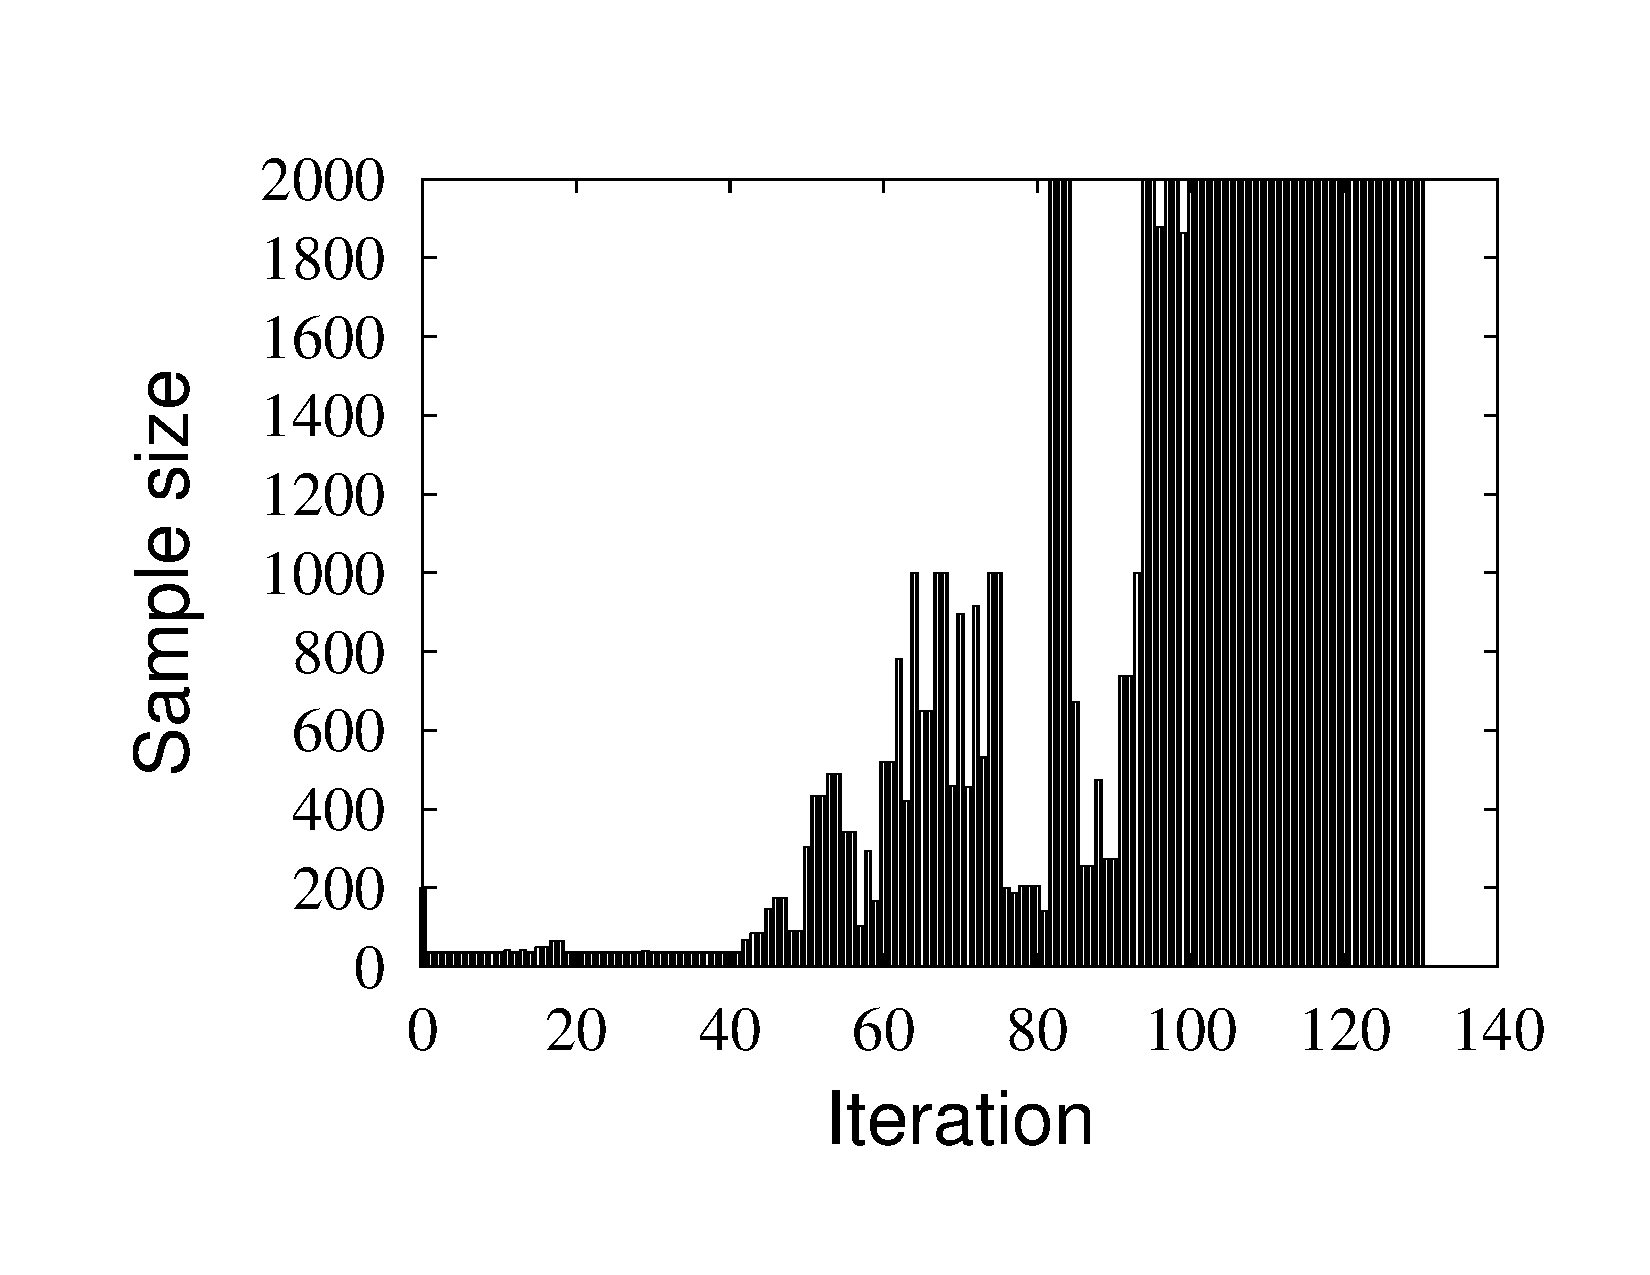
\includegraphics[width=\linewidth]{2000_sample_iter.pdf}
\end{minipage}
\begin{minipage}{0.49\linewidth}
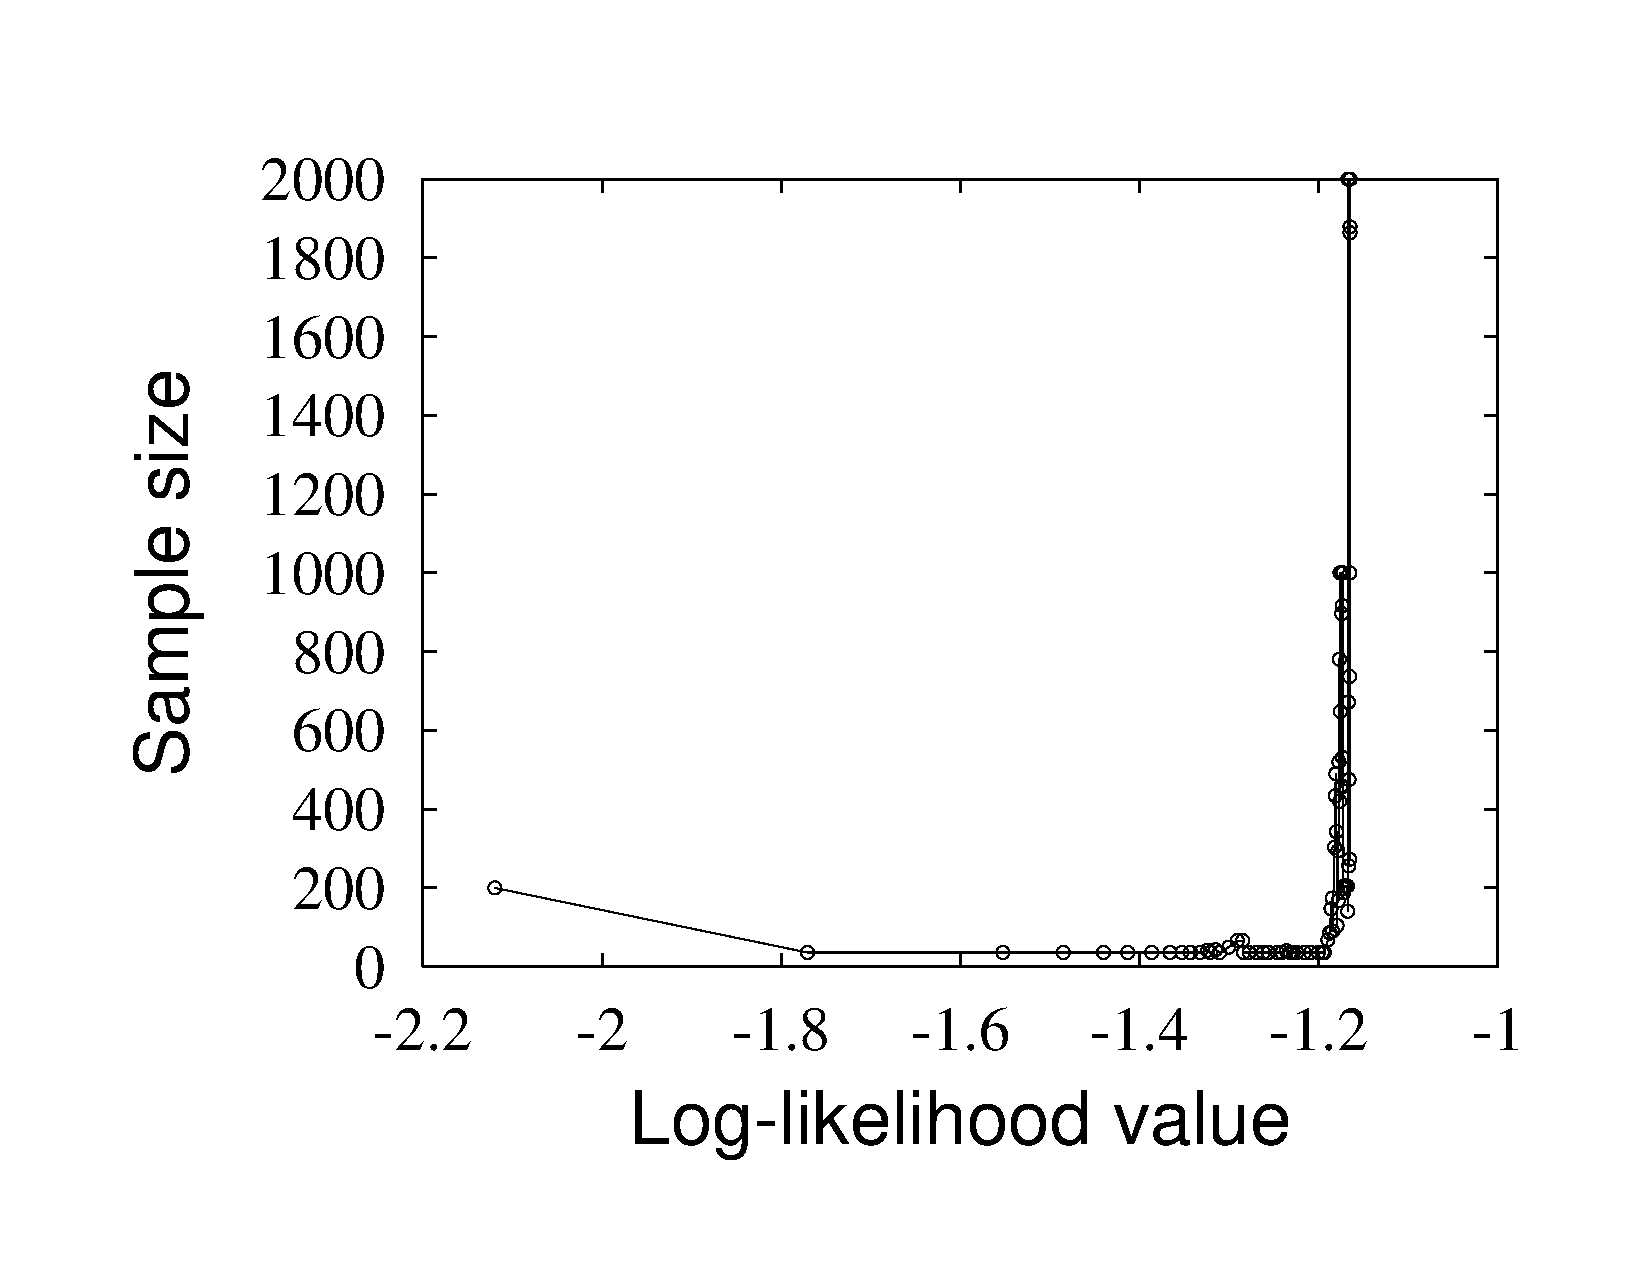
\includegraphics[width=\linewidth]{2000_sample_fct.pdf}
\end{minipage}
\end{center}
\begin{tiny}
{%\red
\hspace*{6.8cm}$\downarrow$\hspace*{3cm}$\downarrow$\\
\hspace*{6.0cm}Starting value\hspace*{1.2cm}Maximum value\\
}
\end{tiny}

\end{frame}

\end{document}